\section{Auswertung}
\label{sec:Auswertung}

\subsection{Bestimmung des Elasitzitätsmodul zweier einseitig eingespannter Stäbe}

\subsubsection{Stab mit quadratischem Querschnitt}

Bei der Messung des Stabes mit rechteckigem Querschnitt, einer Länge 
$L_1= \SI{60}{\centi\meter}$ und einem Gewicht von $m_1 = \SI{464.3}{\gram}$
ergaben sich die Messwerte in Tabelle \ref{tab:Messdaten1}. Dabei ergibt sich 
die Durchbiegung $D$ durch die Differenz von $b_1$ und $b_2$. Der 
Linearisierungsterm ergibt sich mit $Lx²-\frac{x³}{3}$

\begin{table}
\centering
\caption{Biegung eines Stabes mit rechteckigem Querschnitt}
\label{tab:Messdaten1}
\sisetup{table-format=2.1}
\begin{tabular}{c c c c c}
\toprule
$x \,/\, \si{\centi\meter}$ & $b_1 \,/\, \si{\milli\meter}$ & 
$b_2 \,/\, \si{\milli\meter}$ & $D \,/\, \si{\milli\meter}$ &
$Lx²-\frac{x³}{3} \,/\, \SI{e5}{\milli\meter³}$\\
\midrule
 2.5 & -0.005 & 0.060  & 0.065 &   3.323\\
 5.5 & -0.270 & -0.215 & 0.055 &  15.780\\
 8.5 & -0.380 & -0.280 & 0.100 &  36.968\\
11.0 & -0.435 & -0.300 & 0.135 &  60.903\\
13.0 & -0.480 & -0.305 & 0.175 &  83.937\\
15.0 & -0.500 & -0.310 & 0.190 & 110.250\\
17.0 & -0.540 & -0.265 & 0.275 & 139.683\\
19.0 & -0.580 & -0.265 & 0.315 & 172.077\\
21.0 & -0.620 & -0.240 & 0.380 & 207.270\\
23.0 & -0.620 & -0.225 & 0.395 & 245.103\\
25.0 & -0.720 & -0.220 & 0.500 & 285.417\\
27.0 & -0.810 & -0.235 & 0.575 & 328.050\\
29.0 & -0.850 & -0.220 & 0.630 & 372.843\\
31.0 & -0.900 & -0.250 & 0.650 & 419.637\\
33.0 & -0.990 & -0.190 & 0.800 & 468.270\\
35.0 & -1.025 & -0.130 & 0.895 & 518.583\\
37.0 & -1.040 & -0.080 & 0.960 & 570.417\\
39.0 & -1.050 & -0.070 & 0.980 & 623.610\\
41.0 & -1.080 & -0.030 & 1.050 & 678.003\\
42.0 & -1.100 & -0.020 & 1.080 & 705.600\\
43.0 & -1.100 &  0.005 & 1.105 & 733.437\\
44.0 & -1.100 &  0.030 & 1.130 & 761.493\\
45.0 & -1.090 &  0.055 & 1.145 & 789.750\\
46.0 & -1.090 &  0.120 & 1.210 & 818.187\\
47.0 & -1.090 &  0.160 & 1.250 & 846.783\\
48.0 & -1.100 &  0.160 & 1.260 & 875.520\\
49.0 & -1.100 &  0.190 & 1.290 & 904.377\\
49.5 & -1.110 &  0.220 & 1.330 & 918.843\\
\bottomrule
\end{tabular}
\end{table}

Nun wird die Durchbiegung $D$ gegen $Lx²-\frac{x³}{3}$ graphisch aufgetragen
und eine lineare Regressions mittels Python und matplotlib durchgeführt.
Der resultierende Graph ist in Abbildung \ref{fig:plot1} dargestellt.

\begin{figure}
  \centering
  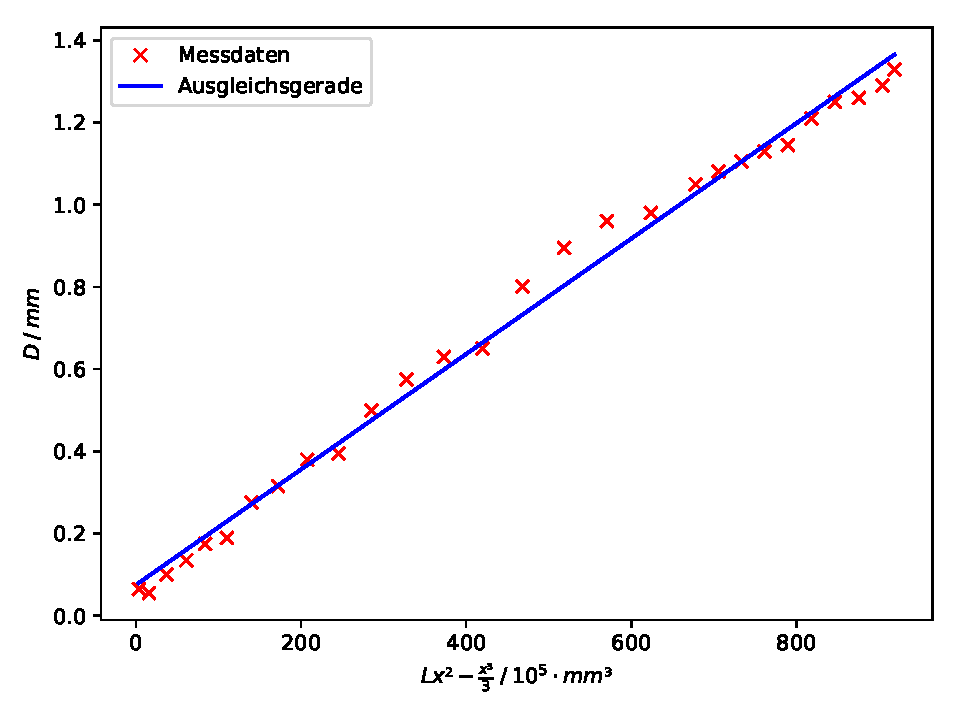
\includegraphics[scale=0.8]{content/plot1.pdf}
  \caption{Durchbiegung mit Regression}
  \label{fig:plot1}
\end{figure}

Die Regression wird mit $D(x) = m_1\cdot x + c_1$ durchgeführt. Dabei ergeben 
sich die Parameter zu: 

\begin{align*}
m_1 &= \SI{0.0140+-0.0002}{1\per\meter²}\\
c_1 &= \SI{0.0752+-0.01364}{\milli\meter}
\end{align*}

Nach Formel \eqref{eqn:Biegung} ergibt sich die Formel: 

\begin{equation*}
E = \frac{F_G}{2m_1\symbf{I}}
\end{equation*}

Hierbei ist $F_G = m_g\cdot g$ mit $m_g = \SI{0.528}{\kilo\gram}$ und 
$g = \SI{9.81}{\meter\per\second\squared}$. Das Flächenträgheitsmoment
ergibt sich nach Formel ... zu $\frac{1}{12} \SI{e4}{\milli\meter⁴}$. 
Das Elastizitätsmodul ist also gegeben durch: 

\begin{equation*}
E = \SI{2.220+-0.032e5}{\newton\per\milli\meter²}
\end{equation*}

Der statische Fehler ergibt sich mit der Gaußschen Fehlerfortpflanzung zu: 

\begin{equation*}
\Delta E = \frac{\partial E}{\partial m_1}\cdot \Delta m_1 
= \frac{-F_G}{2\symbf{I}m²} \cdot \Delta m_1
\end{equation*}

Es scheint sich demnach bei dem Material um Stahl zu handeln, dessen 
Elasitzitätsmodul bei $E=\SI{220000}{\newton\per\milli\meter²}$ [1] liegt.

\subsubsection{Stab mit zylindrischem Querschnitt}

Das Verfahren läuft analog mit dem runden Stab mit $L = \SI{55.2}{\centi\meter}$.
Die entsprechenden Messdaten finden sich in Tabelle \ref{tab:Messdaten2}. 

\begin{table}
\centering
\caption{Biegung eines Stabes mit zylindrischem Querschnitt}
\label{tab:Messdaten2}
\sisetup{table-format=2.1}
\begin{tabular}{c c c c c}
\toprule
$x \,/\, \si{\centi\meter}$ & $b_1 \,/\, \si{\milli\meter}$ & 
$b_2 \,/\, \si{\milli\meter}$ & $D \,/\, \si{\milli\meter}$ &
$Lx²-\frac{x³}{3} \,/\, \SI{e5}{\milli\meter³}$\\
\midrule
 2.5 &  0.000 & 0.170 & 0.170 &   3.398\\
 5.5 & -0.110 & 0.050 & 0.160 &  16.143\\
 8.5 & -0.310 & 0.020 & 0.330 &  37.835\\
11.0 & -0.395 & 0.030 & 0.425 &  62.355\\
13.0 & -0.455 & 0.065 & 0.520 &  85.965\\
15.0 & -0.510 & 0.013 & 0.523 & 112.950\\
17.0 & -0.570 & 0.270 & 0.840 & 143.151\\
19.0 & -0.600 & 0.400 & 1.000 & 176.409\\
21.0 & -0.645 & 0.560 & 1.205 & 212.562\\
23.0 & -0.710 & 0.775 & 1.485 & 251.451\\
25.0 & -0.680 & 0.985 & 1.665 & 292.917\\
27.0 & -0.650 & 1.150 & 1.800 & 336.798\\
29.0 & -0.630 & 1.565 & 2.195 & 382.935\\
31.0 & -0.600 & 1.700 & 2.300 & 431.169\\
33.0 & -0.560 & 2.000 & 2.560 & 481.338\\
35.0 & -0.560 & 2.260 & 2.820 & 533.283\\
37.0 & -0.555 & 2.460 & 3.015 & 586.845\\
39.0 & -0.550 & 2.820 & 3.370 & 641.862\\
41.0 & -0.550 & 3.050 & 3.600 & 698.175\\
42.0 & -0.550 & 3.200 & 3.750 & 726.768\\
43.0 & -0.550 & 3.385 & 4.935 & 755.625\\
44.0 & -0.550 & 3.500 & 4.050 & 784.725\\
45.0 & -0.540 & 3.630 & 4.170 & 814.050\\
46.0 & -0.520 & 3.780 & 4.300 & 843.579\\
47.0 & -0.500 & 3.930 & 4.430 & 873.291\\
48.0 & -0.480 & 4.030 & 4.510 & 903.168\\
\bottomrule
\end{tabular}
\end{table}

Trägt man nun erneut $D$ gegen $L\cdot x²-\frac{x³}{3}$ auf und führt eine
Ausgleichsrechnung mittels matplotlib durch ergibt sich Abbildung \ref{fig:plot2}. 

\begin{figure}
  \centering
  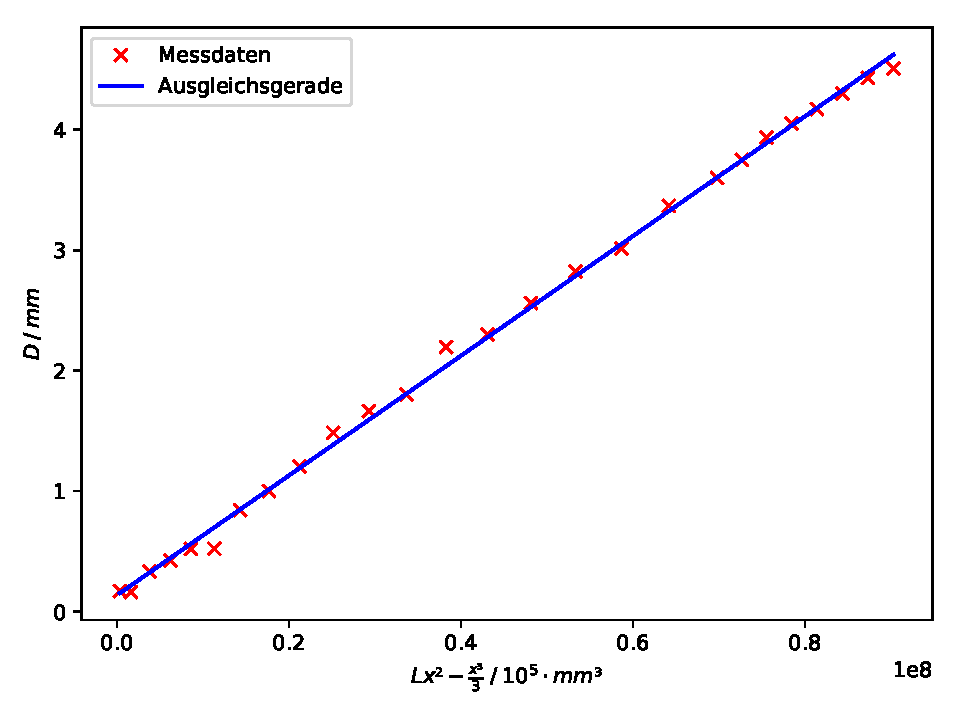
\includegraphics[scale=0.8]{content/plot2.pdf}
  \caption{Durchbiegung mit Regression}
  \label{fig:plot2}
\end{figure}

Die Regressionsparamter ergeben sich dabei zu: 

\begin{align*}
m_2 &= \SI{0.0497+-0.0004}{1\per\meter²}\\ 
c_2 &= \SI{0.1362+-0.0232}{\milli\meter}
\end{align*}

Bei diesem Stab ist das Flächenträgheitsmoment nach Formel ... 
gegeben durch $\frac{\pi}{64} \si{\centi\meter⁴}$.
Schließlich ergibt sich für das Elasitzitätsmodul $E$ wie oben mit Formel 
\eqref{eqn:Biegung} und durch das Flächenträgheitsmoment:

\begin{equation*}
E = \SI{1.037+-0.008e5}{\newton\per\milli\meter²}
\end{equation*}